\documentclass[12pt]{article}

\usepackage{fullpage}
\usepackage{graphicx, rotating, booktabs} 
\usepackage{times} 
\usepackage{natbib} 
\usepackage{indentfirst} 
\usepackage{setspace}
\usepackage{grffile} 
\usepackage{hyperref}
\usepackage{adjustbox}
\usepackage{amsmath}
\usepackage{siunitx}
\usepackage{multirow}
\setcitestyle{aysep{}}


\singlespace
\title{\textbf{Democracy and the Sources of Alliance Treaty Depth}}
%\author{Joshua Alley\footnote{Graduate Student,
%Department of Political Science, Texas A\&M University.}}
\date{}

\bibliographystyle{apsr}

\begin{document}

\maketitle 

\doublespace 

\begin{abstract}
Why do states make commitments of defense coordination and cooperation in military alliance treaties? 
I argue that states use treaty depth to increase alliance credibility when domestic political institutions generate audience cost concerns, but allow states to accept greater foreign entanglement. 
Because democratic leaders fear paying high domestic audience costs to avoid entrapment, and voters have little concern with entanglement short of war, they use treaty depth to reassure allies. 
Unlike depth, unconditional military support generates audience cost concerns. 
Thus, democratic alliance leadership increases treaty depth but decreases the likelihood of unconditional military support. 
I test this claim on offensive and defensive alliances from 1816 to 2007 and illustrate the theoretical mechanisms by examining NATO. 
I find that democratic institutions in the most capable alliance member increase treaty depth, but have a mixed impact on unconditional military support. 
The argument and findings challenge claims that democracies prefer limited alliance commitments. 
\end{abstract}


\newpage 


\section{Introduction}


% Start with question and motive 
Why do states make deep alliance treaties? 
Around half of all alliances with active military support obligations also include commitments of peacetime defense cooperation and policy coordination \citep{Leedsetal2002}. 
Despite the prevalence of alliance treaty depth, we have little idea when states add depth to their alliances and why they might prefer depth to other means of establishing credible commitments.
Understanding treaty depth is also worthwhile because depth changes alliance politics. 
Greater credibility encourages non-major power members of deep alliances to reduce military spending \citep{Alley2020}.  
Thus, treaty depth shapes credibility and the distribution of military spending among alliance members. 


% Describe question and contribution of the paper
In this paper, I explain why states make deep alliance treaties. 
Deep alliances formalize extensive defense cooperation by requiring additional military policy coordination and cooperation beyond a promise of military intervention. 
While shallow alliances offer arms-length military support, deep treaties lead to closer ties between alliance members. 
Common sources of depth include an integrated military command, military aid, a common defense policy, basing rights, international organizations, specific capability contributions and companion military agreements. 


I argue that states use treaty depth to increase the credibility of their alliance commitments while managing entrapment risk.
I start with the premise that treaty depth and unconditional promises of military support are two costly ways states can increase the credibility of their alliance commitments.
I then argue that domestic political institutions affect which credibility source states prefer by shaping the audience costs of violating military support promises.
Because democratic leaders have high audience costs from treaty violation, they use deep alliance treaties to signal credible commitment and avoid entrapment.
Leaders are free to form deep alliances because voters rarely scrutinize foreign entanglements short of war. 
Unconditional promises of military support commit to military intervention regardless of circumstances.  
Unconditional military support promises force leaders to violate the alliance and pay audience costs if an ally invokes the alliance and they want to stay out.
As a result, democracies often make conditional alliance commitments to avoid paying audience costs \citep{Mattes2012, Chibaetal2015}.
Therefore, I expect that democracies will often design deep alliances with conditional promises of military support. 


I test the argument with a statistical analysis of offensive and defensive alliances from 1816 to 2007 and then examine the theoretical mechanisms in the case of NATO.
I estimate a series of statistical models to assess the association between democratic institutions in the most capable alliance member and treaty design, including bivariate models that adjust for correlated errors in treaty depth and unconditional military support equations \citep{Braumoelleretal2018}. 
I focus on democratic institutions in the most capable member because these alliance leaders have substantial influence on treaty design. 
After examining the overall effect of democracy, I disaggregate democratic institutions into competitive elections, open political competition, and executive constraints and find that elections drive the positive relationship between democracy and treaty depth. 
In general, there is consistent evidence that alliances with a democratic leader have higher treaty depth.
I find limited evidence that democratic alliance leadership decreases the probability of unconditional military support, however, because elections and executive constraints have offsetting effects. 


% Two Paras on the gap I fill 
This paper contributes to knowledge of alliance treaty design and how domestic politics affects alliance choices.
Scholars have long acknowledged a connection between democracy and alliances \citep{LaiReiter2000, GiblerWolford2006, Mattes2012, Warren2016, McManusYarhi-Milo2017}. 
Connecting domestic institutions and treaty depth addresses an important gap in the literature. 
The process of alliance treaty negotiation and design is understudied \citep{Poast2019a}, and there is little research on treaty depth because the nascent alliance treaty design literature emphasizes conditions on military support.
Existing research identifies entrapment concerns \citep{Kim2011, Benson2012} and democratic alliance membership \citep{Mattes2012, Chibaetal2015} as two notable sources of conditional obligations.\footnote{\citet{FjelstulReiter2019} supplement research on conditionality by arguing that democracies use incomplete alliance contracts to limit audience costs.} 


Two studies of alliance treaty design examine similar concepts to treaty depth, but both have important limitations.   
First, \citet{Mattes2012} finds that members of symmetric bilateral alliances where one partner has history of violation are more likely to use military institutionalization to increase treaty reliability. 
This paper makes an important contribution, but it does not differentiate between the costs and benefits of issue linkages, military institutionalization and conditional obligations the argument, only analyzes bilateral alliances, and uses a military institutionalization measure \citep{LeedsAnac2005} that understates the amount of variation in treaty depth.  
Second, while checking the validity of a latent measure \citet{BensonClinton2016} find that foreign policy agreement, major power involvement and treaty scope increase depth. 
Benson and Clinton define depth as how costly alliance obligations are in general, however, so their latent measure of depth includes secrecy and issue linkage and captures a broader concept than military cooperation. 
Neither study explains why states prefer different sources of alliance credibility. 


Therefore, we still do not understand why alliance members add treaty depth when there are multiple ways to establish credible commitments. 
To explain deep alliances, I compare treaty depth and unconditional military support.  
Although treaty depth and unconditional military support increase alliance credibility, depth leads to foreign entanglement, while unconditional support increases entrapment risk. 
Domestic political institutions shape whether entrapment or entanglement is more concerning by changing leaders' foreign audiences, and thus determines which source of credibility leaders prefer. 


% implications: 
My argument and findings have two implications. 
First, they contradict claims that democracies prefer limited alliance commitments \citep{Mattes2012, Chibaetal2015, FjelstulReiter2019}. 
After finding that democracies are more likely to make conditional promises of military support, \citet{Chibaetal2015} write that ``domestic costs can make democratic states wary of engaging in agreements requiring broad and/or deep cooperation.'' 
My argument suggests that even if democracies screen the breadth of their commitments, they form deeper alliances on other dimensions.\footnote{This paper examines a slightly different sample than earlier research, which sometimes includes consultation pacts. I focus on alliances with active military support.}  
Furthermore, I add to the rich literature on domestic politics and international cooperation e.g. \citep{DownesRocke1995, Fearon1998, Leeds1999, MattesRodriguez2014}. 
If democracies reassure partners with deep alliance commitments, audience costs may push democracies to undertake strong international commitments with less electoral salience.\footnote{For example, in environmental agreements, democracies use soft law commitments to avoid audience costs of violation \citep{BoehmeltButkute2018}, but there may be other agreements that are less salient and more binding.} 


% roadmap for the paper 
The paper proceeds as follows. 
In the next section, I lay out the argument and hypothesis. 
Then I summarizes the data and research design. 
After this, I describe the results and detail the alliance treaty design process in NATO.
In the final section I summarize the results and offer some concluding thoughts. 


\section{Argument}


In this argument, I first situate treaty depth in a general alliance politics framework.  
After that, I offer a general explanation of the costs and benefits of treaty depth, relative to unconditional military support. 
Based on the different costs and risks of treaty depth and unconditional military support, I then detail why I expect that democracies often add depth, but are less likely to offer unconditional support. 


Alliances are self-enforcing contracts or institutions where states promise military intervention \citep{Leedsetal2002, Morrow2000}. 
When faced with external threats in an anarchic international system, states form alliances to aggregate military capability and secure their foreign policy interests \citep{Altfield1984, Smith1995, Snyder1997, FordhamPoast2014}.
Alliance participation has several costs and benefits.
Beyond the benefit of possible military support, alliances also clarify international alignments \citep{Snyder1990} and support economic ties \citep{Gowa1995, Li2003, Long2003, Fordham2010, WolfordKim2017}.  
The costs of alliance participation include opportunism and lost foreign policy autonomy \citep{Altfield1984, Morrow2000, Johnson2015}. 
Opportunism in alliances has three forms; abandonment \citep{Leeds2003a, BerkemeierFuhrmann2018}, entrapment in unwanted conflicts \citep{Snyder1984}, and free-riding \citep{Morrow2000}.


% process of alliance negotiations: establishing a credible commitment. 
To form an alliance, states must have similar foreign policy interests \citep{Morrow1991, Smith1995, FordhamPoast2014}, especially in their proposed war plans \citep{Poast2019a}. 
The treaties that formalize promises of military support take many forms \citep{Leedsetal2000, Leedsetal2002, Benson2012, BensonClinton2016}. 
Treaty design shapes the costs and benefits of treaty participation and addresses potential opportunism. 
Alliance members use formal commitments to increase the credibility of military intervention promises \citep{Morrow2000}. 
In the face of abandonment concerns, alliance members and other states use the costs of the alliance commitment to assess reliability. 
While alliance formation alone adds some credibility, treaty depth and unconditional promises of military support are further costly commitments that add credibility, albeit in different ways.  


% conditions: balance credible commitment and entrapment 
Unconditional alliances promise military intervention under any circumstance. 
These promises generate credibility in a way that increases the risk of entrapment in unwanted conflicts, however. 
If an ally invokes a treaty when a state would rather stay out, states must choose between fighting in an unwanted war, or paying the reputational \citep{Gibler2008, Crescenzietal2012} and audience \citep{Fearon1997} costs of treaty violation.
When alliance members fear divergent allied interests will create this entrapment or violation dilemma, they constrain military support to specific circumstances \citep{Kim2011, Benson2012}.\footnote{Such deliberate alliance design means clear instances of entrapment are rare \citep{Kim2011, Beckley2015}.} 
Conditional alliances limit promises of intervention to particular regions, conflicts, or instances of non-provocation \citep{Leedsetal2000}. 
Conversely, offering unconditional military support indicates more shared foreign policy interests and less fear of entrapment.
Under unconditional commitments alliance members hazard the costs of fighting, entrapment or treaty violation in more circumstances, which adds credibility.  


Unconditional promises of military support reflect substantial foreign policy agreement.
Alliances face a time-inconsistency problem, however \citep{LeedsSavun2007}. 
Although treaties fix conditions on military support, foreign policy interests change. 
If a partner calls on a state to fight in an unwanted conflict after interests shift, states must bear either entrapment or audience and reputation costs.
When audience costs are less costly than fighting, which is usually the case, states will violate the treaty and pay the audience costs.\footnote{This may be another reason that entrapment, or fighting in unwanted conflict, is rare.}    
But states with high audience costs will be more sensitive to having the alliance invoked in unwanted conflicts, because violation is more costly. 
Therefore, states with high audience costs will be less likely to offer unconditional military support. 


% Part 2: depth 
Treaty depth offers another way to establish credibility with less risk of having to pay audience costs to avoid entrapment. 
Deep alliances increase credibility and allow states to manage entrapment risk at the cost of foreign entanglement. 
Depth adds to the perceived reliability of an alliance by providing opportunities for states to fulfill treaty obligations in peacetime \citep{Morrow1994}. 
Implementing deep treaty obligations is a sunk cost signal of commitment.
Observing that alliance members adhere to peacetime promises suggests that they will also honor promises of military support. 


Depth limits the risk of entrapment in two ways. 
First, depth provides indications of changing foreign policy interests.   
Failure to implement deep alliance provisions provides an observable signal of foreign policy divergence.
Thus, deep alliances can generate warnings about foreign policy changes before states invoke military support obligations. 
Second and more importantly, deep alliances increase states' influence over allied conflict decisions.  
Bases, joint organization and policy coordination are all potential checks on entrapment.
For example, the United States used deep alliance ties with South Korea to control ``adventurism'' by the Rhee regime \citep{Cha2016}. 
Coordinating policies over time allows states to ensure that their joint war plans still line up, and that no member faces prohibitive abandonment or entrapment risks.  
Thus, even if credibility from treaty depth create moral hazard \citep{Benson2012, FuhrmannSechser2014}, depth also provides ways to assess allied interests and constrain such opportunism. 


% depth has a different cost: FP autonomy
Treaty depth mitigates the reliability and entrapment dilemma, but increases foreign entanglement. 
Lost foreign policy autonomy is the other key cost of alliance participation besides opportunism, and deep alliances reduce foreign policy autonomy more than other alliances.
Cooperating and coordinating policy with allies reduces the ability of states to make unilateral decisions. 
There are also practical hurdles to unwinding foreign bases, international institutions and integrated military commands. 
Binding allies closely with treaty depth increases credibility and checks entrapment, but close ties reduce alliance members' freedom of action. 


% summarize difference in costs (candidate to cut if needed) 
To summarize the argument so far, although depth and unconditional military support both increase alliance credibility, they have different costs. 
Unconditional military support raises the risk of paying audience costs or entrapment. 
Conversely, treaty depth increases credibility with costly cooperation, which manages entrapment risk, but leads to greater foreign entanglement.   


% Combine the two & separate out the role of FP audiences
Relative concern with entrapment or foreign entanglement shapes how states establish credible commitments in alliance treaty design. 
When state leaders fear paying the audience costs of treaty violation to avoid entrapment and can accept foreign entanglement, they will form deep alliances with conditional promises of military support.\footnote{This argument focuses on when states might prefer depth to unconditional military support. Prospective alliance members could also make an arms-length alliance commitment with neither depth nor unconditional military support, or use treaty depth to address time-inconsistency problems with unconditional military support.}
Concern with audience costs and foreign entanglement depends on leaders' foreign policy audiences.  
Domestic political institutions shape the foreign policy audiences that leaders depend on to continue in office \citep{Weeks2008}. 
In democracies, voters are leaders' key audience for foreign policy decisions.  
Due to high audience costs of violating military support promises and low public concern with foreign entanglement short of military intervention, I expect that alliances with democratic leaders will be more likely to have high depth and conditional military support. 



\subsection{Democratic Alliance Leadership and Treaty Design}


% Talk about voters
Democracies use treaty depth to reassure partners because depth increases the perceived reliability of their alliances while avoiding the dilemma of entrapment or paying audience costs. 
Violating international promises can create audience costs for democratic leaders.
Democratic leaders fear that if they violate international commitments, voter disapproval could lead to their removal from office.  
In alliance politics, audience costs could occur when leaders violate treaty obligations, so long as the public is paying attention to the foreign policy issue \citep{Slantchev2006, PotterBaum2014} and prefers compliance \citep{Chaudoin2014, KertzerBrutger2016}.  


Military support commitments can generate public attention and audience costs in democracies. 
Audience costs increase as crises escalate \citep{Tomz2007}, so promises of military support and a possible military intervention are salient to the democratic public.  
\citet{Baum2002} shows that even otherwise inattentive individuals often receive information about foreign policy crises through entertainment news. 
Given public attention to a foreign crisis, an unconditional promise of military support exposes democratic leaders to paying audience costs if they do not want to intervene. 
As a result, entrapment through unconditional military support is concerning for democratic leaders, as they cannot avoid fighting without audience costs.
Limiting alliance commitments through conditional military support reduces audience costs because it is easier for democratic leaders to claim that the conditions for intervention were not met, or that new information eliminates intervention obligations \citep{LevenduskyHorowitz2012}. 


Treaty depth mitigates the audience cost concerns of democratic leaders by managing exposure to unwanted conflicts.  
Deep alliances reduce the risk that if the alliance is invoked, leaders would prefer to stay out and bear audience costs for doing so. 
Although depth leads to foreign entanglement, democratic audiences are less likely to be concerned with foreign entanglement short of war.
The public in democracies lacks substantial foreign policy information, so foreign entanglements from treaty depth have limited salience in domestic politics. 
Few voters will have much information about defense cooperation with allies. 
Although foreign policy elites may dispute deep alliance commitments or violations of treaty depth, such dissent is unlikely to translate into meaningful public opposition and electoral concerns.


% How do allies respond?
Despite its limited role in the domestic politics of democracies, treaty depth is salient in international politics.
Allied states and potential adversaries can gather useful information from treaty depth. 
By including peacetime costs in a deep treaty, alliance members signal alliance reliability. 
Implementing costly promises of military aid, bases, or policy coordination indicates commitment. 
This increases allied confidence that democracies will honor their treaty obligations. 
Therefore, democracies can use treaty depth to signal international commitment with less exposure to domestic audience costs and electoral scrutiny. 


% analogous to optimal obfuscation in trade policy
The way democracies use treaty depth in alliances is analogous to their emphasis on non-tariff barriers in trade policy.
\citet{Kono2006} argues that because non-tariff barriers are more complex, voters lack sufficient information about their impact on consumer prices.
Tariffs, on the other hand, translate directly into prices in ways that are easy to understand.
The complexity of non-tariff barriers makes them less vulnerable to electoral attack, so democracies engage in ``optimal obfuscation'' and substitute non-tariff barriers for tariffs. 
In the same way, unconditional promises of military support and treaty depth both affect international relations, but the former is salient for voters and the latter is not. 
Unconditional military support and related violations are easy for voters to grasp, but treaty depth is not. 
Therefore, democratic leaders can use treaty depth to manage international politics with fewer domestic political consequences.


% What is it exactly about democracies
Three components of democratic institutions could generate audience cost concerns. 
Open elections for leadership, open political competition and legal constraints on executive action are three possible sources of audience costs in democracies. 
Selecting leaders through elections makes leaders accountable to voters. 
Political competition allows opposition groups to hold leaders to account for foreign policy shortcomings \citep{PotterBaum2014}. 
Democratic leaders also face legal constraints on their foreign policy, and violating these restraints could generate audience costs. 
I examine the relative weight of these three institutional mechanisms in the empirical analysis.  


% What about different types of autocracies? 
This argument uses limited audience concerns and reassurance benefits of treaty depth to explain why democracies often form deep alliances. 
What about autocracies? 
Some autocratic leaders, especially in single-party states, also face high audience costs from domestic elites for backing down in military conflicts \citep{Weeks2014}.
Domestic elites in single party states are a different audience than the public in democracies, however.  
Party elites are more informed about foreign policy than the public in democracies, so they are more likely to scrutinize foreign entanglements and impose costs on leaders that violate deep alliance obligations. 
In general, no autocratic audience has the same combination of limited foreign policy information and high audience costs of military intervention as democracies.
Single-party and military regime leaders face an informed domestic elite, and personalist leaders lack a foreign policy audience that can impose costs. 
Therefore, assuming that all autocracies are equivalent, relative to democracies is sufficient for this paper.\footnote{Examining heterogeneity among autocracies in alliance treaty design is an interesting subject for future research, however.} 


% Sources of democratic influence in alliance negotiations. 
Of course, democracies may not get what they prefer in alliance negotiations. 
More capable states have greater influence on alliance negotiations \citep{Mattes2012}, because their partners lose out on more foreign policy benefits if they are out of the alliance.
The most capable state is often the alliance ''leader,'' and their preferences carry more weight. 
Therefore, to understand how democracy shapes alliance treaty design, I conceptualize democratic influence in terms of the political regime type of the most capable alliance member. 


% express the key hypothesis
Because depth adds credibility but limits exposure to audience costs and voters have little concern with foreign entanglement, democracies will often design deep alliance treaties. 
As the democracy of the most capable alliance member at the time of treaty formation increases, treaty depth will increase. 


\begin{quote}
\textsc{Treaty Depth Hypothesis: As the democracy of the most capable alliance member at the time of formation increases, alliance treaty depth will increase.}
\end{quote} 


% End with an established result: democracy and conditional obligations
I also expect that democratic alliance leadership will reduce the probability of unconditional military support, because backing out of a promised military intervention generates substantial audience costs. 
This second claim is based on existing arguments and findings. 
\citet{Mattes2012} and \citet{Chibaetal2015} both show that democracies are more likely to design conditional alliances. 
They attribute this finding to higher audience costs from violating international commitments in democracies. 
Because democratic leaders face substantial audience costs, they make limited commitments that are easier to fulfill. 
Based on this logic, more democratic institutions in the most capable member when the alliance formed should reduce the probability of unconditional military support.


\begin{quote}
\textsc{Unconditional Military Support Hypothesis: As the democracy of the most capable alliance member at the time of formation increases, the probability that the alliance offers unconditional military support will decrease.}
\end{quote} 


% Discuss the combination
Depth substitutes for unconditional obligations in democratic alliances.  
Because allied states understand the limits of conditional alliances, they may fear challenges \citep{Smith1995}. 
But even if conditional military support reduces the credibility of democratic alliances, treaty depth provides further credibility. 
Thus, depth reassures the allies of democracies, who might otherwise have reliability concerns from conditional military support. 


I expect that democratic alliance leadership will increase treaty depth, but reduce the likelihood of unconditional military support.
In the next section, I describe how I test this claim about the association between democratic alliance leadership and alliance treaty design with a series of statistical models. 
I first describe the key variables in the analysis, then provide more detail on the estimation strategy.


\section{Research Design}


% start with data
To examine my prediction that democracies prefer deep and conditional alliances, I employ data from the Alliance Treaty Obligations and Provisions Dataset \citep{Leedsetal2002}. 
The sample includes 289 alliances with either offensive or defensive obligations, which is the set of treaties with active military support.\footnote{Results are robust to adjusting for non-random selection into alliances. See the appendix for details.} 
I measure treaty depth with a semiparametric mixed factor analysis of eight ATOP variables \citep{Murrayetal2013}.
Unlike other measures, this approach captures the full spectrum of variation in defense cooperation across alliances, as it is more flexible than ordinal measures \citep{LeedsAnac2005} and more focused on defense cooperation than another latent measure \citep{BensonClinton2016}.\footnote{See the appendix for results with measures by \citet{LeedsAnac2005} and \citet{BensonClinton2016}, which lead to similar inferences. I also discuss the relative advantages of my measure in more detail.}
My depth measure is essentially a weighted combination of ATOP's defense policy coordination, military aid, integrated military command, formal organization, companion military agreement, specific contribution, and bases variables, where the weights are estimated by the measurement model.  
All eight variables increase alliance treaty depth, but defense policy coordination and an integrated command add the most to depth, as shown in the top panel of \autoref{fig:loadings-measure}. 


\begin{figure}[hbtp]
\centering
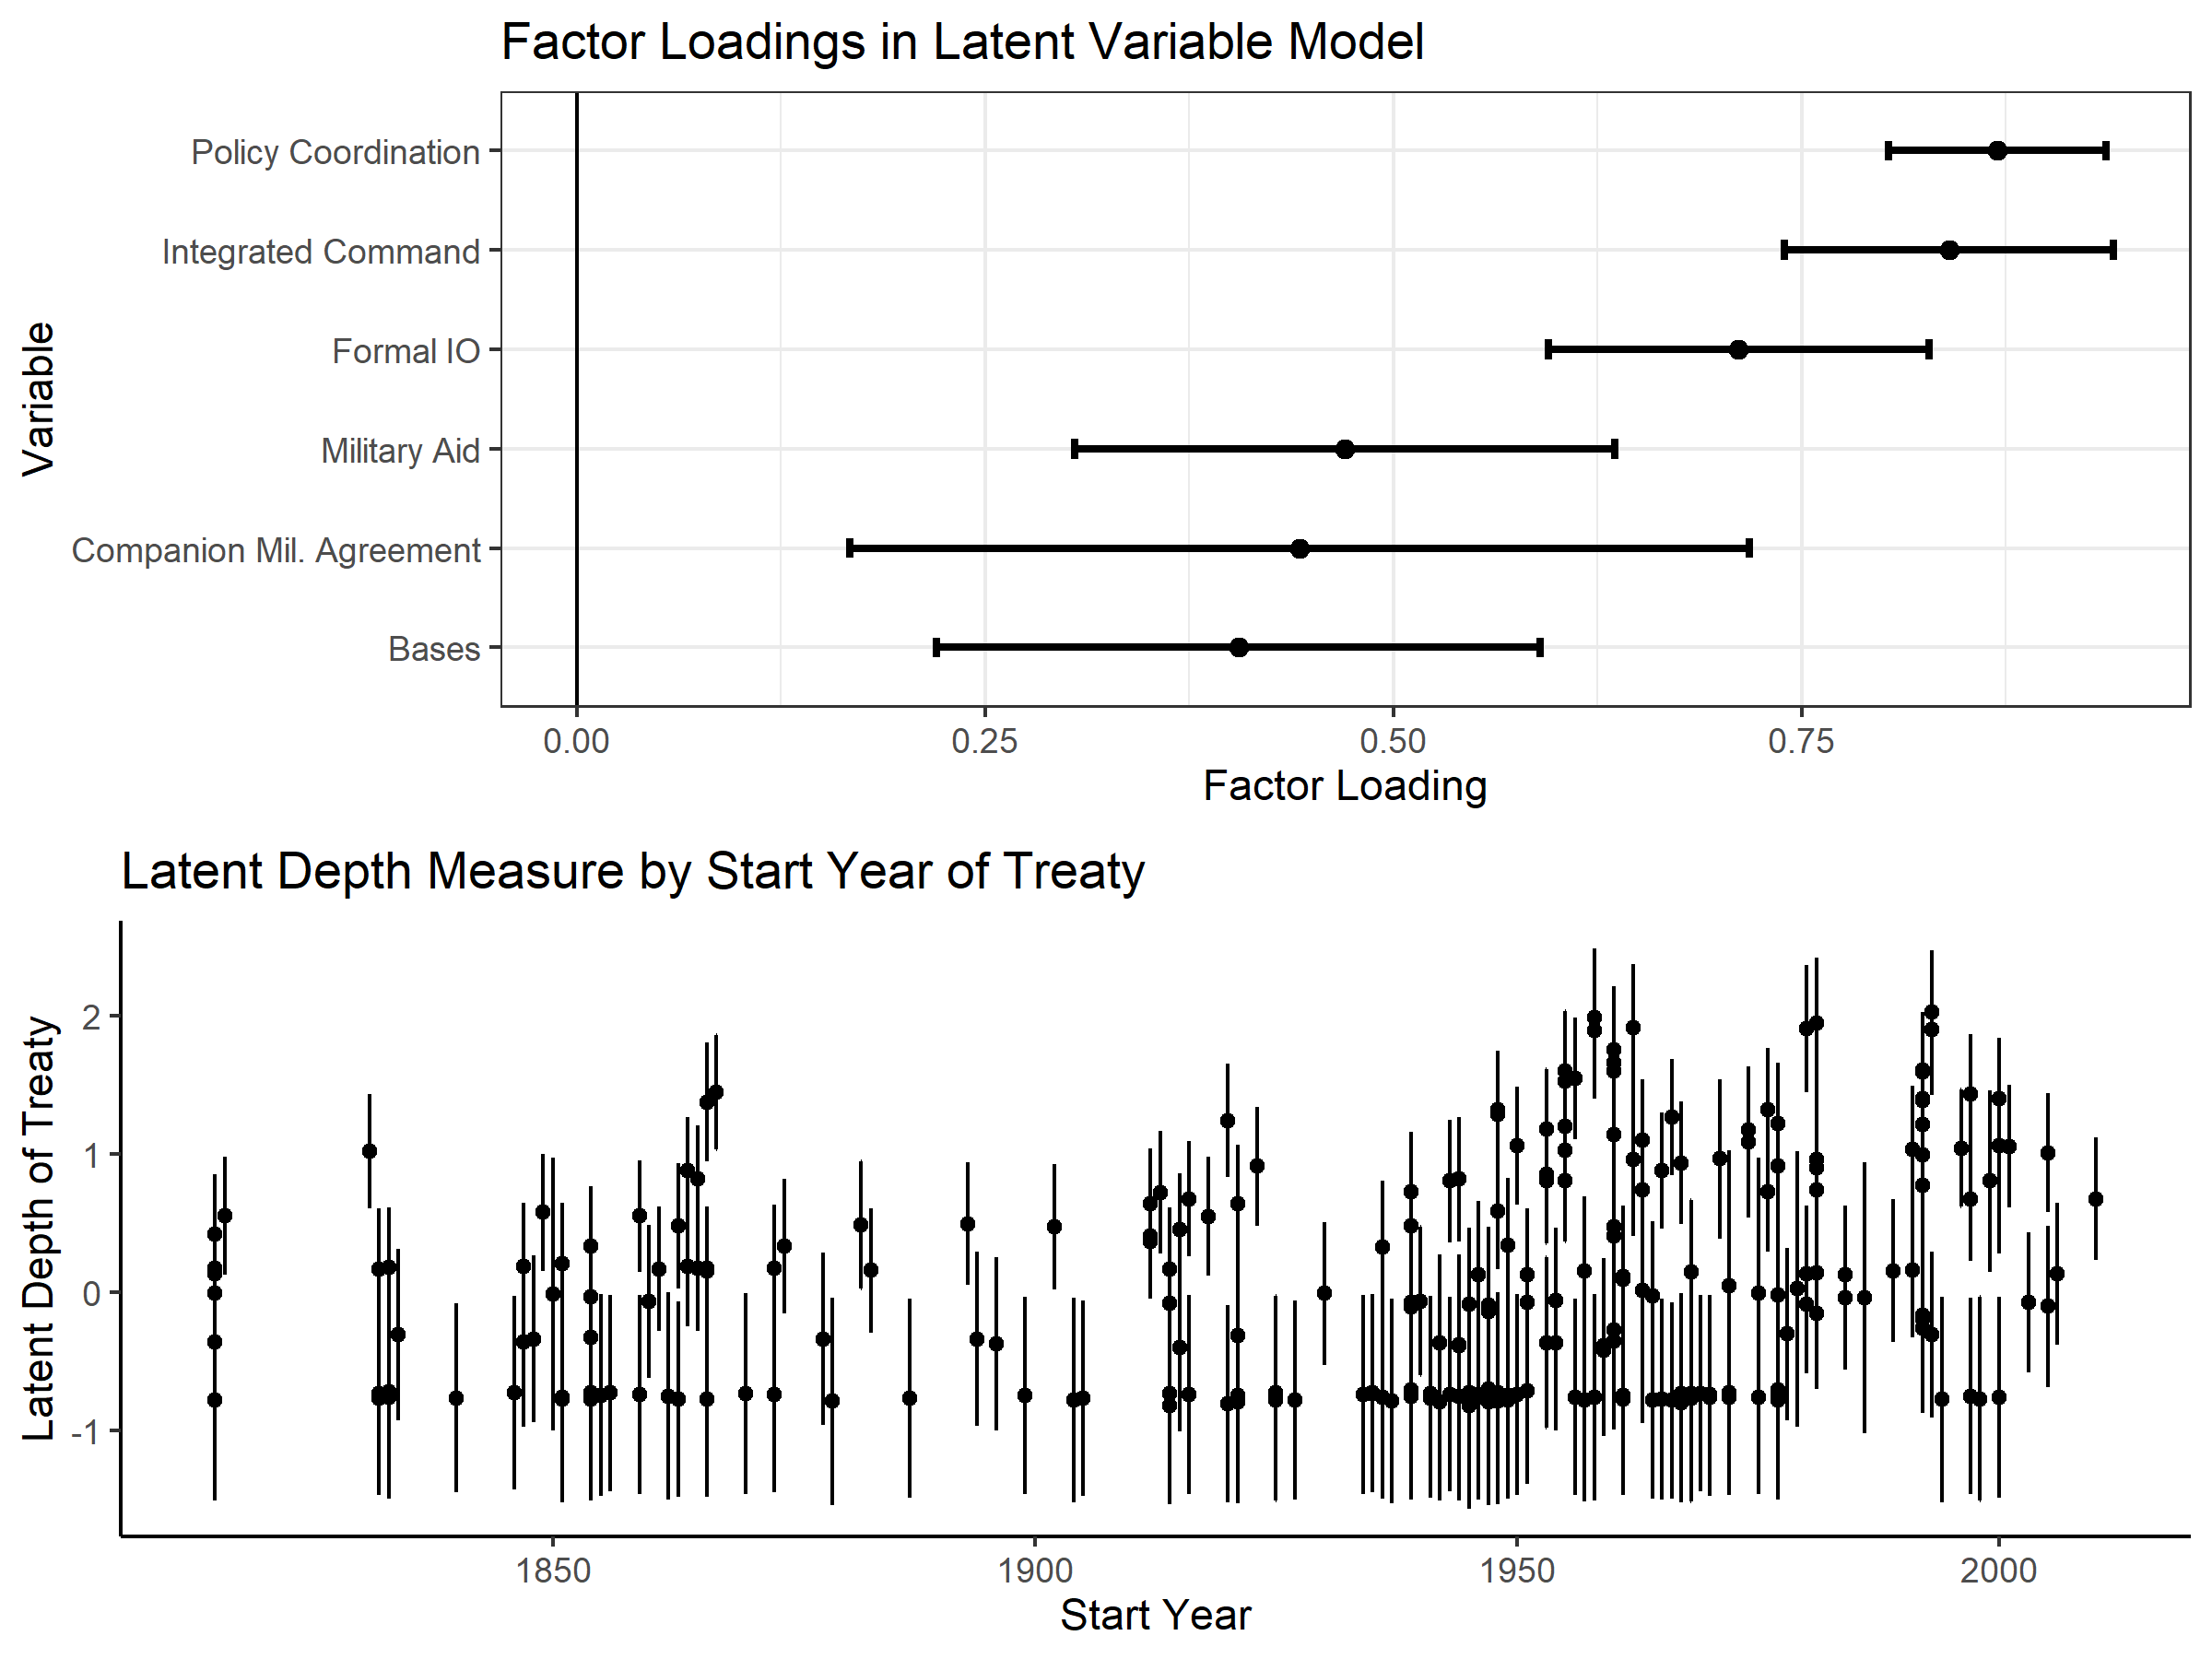
\includegraphics[width=0.95\textwidth]{../figures/loadings-measure.png}
\caption{Factor Loadings and posterior distributions of latent alliance treaty depth measure. Estimates from a semiparametic mixed factor analysis of offensive and defensive ATOP alliances from 1816 to 2007.}
\label{fig:loadings-measure}
\end{figure}


The measurement model predicts each alliance's treaty depth using the factor loadings. 
The bottom panel of \autoref{fig:loadings-measure} summarizes the posterior distributions of the latent treaty depth measure for every alliance in the data. 
There is substantial variation in alliance treaty depth. 
Around half of all formal alliance treaties have some depth, and depth varies widely across alliances.
In the analysis, I measure treaty depth using the mean of the latent depth posterior for each alliance. 
The posterior mean captures the central tendency of latent treaty depth, and I show in the appendix that results are robust to accounting for uncertainty in the latent measure. 


The other outcome variable is a dummy indicator of unconditional military support. 
Using ATOP's information on whether defensive or offensive promises are conditional on specific locations, adversaries, or non-provocation, I set this variable equal to one if the treaty placed no conditions on military support.
123 of 289 alliances offer unconditional military support. 


The key independent variable is the democracy of the most capable alliance member in the year of alliance formation. 
I use the Polity2 (revised combined Polity score) measure of political institutions to measure democracy, and code the alliance leader as the state with the largest CINC score \citep{SingerCINC1988}.
This measure emphasizes the influence of the most capable alliance member and captures the domestic institutions and potential sensitivity of that state to audience costs and entrapment.\footnote{I find similar results with a model that uses the proportion of democracies as the key independent variable, and report them in the appendix. The proportion of democracies measures the prevalence of democratic membership, and has a strong positive correlation with the democracy of the most capable member.}    


After estimating the association between alliance leader Polity scores and treaty design, I break the democracy measure into three components to assess the effects of different democratic institutions.  
The Polity measure aggregates executive recruitment, political competition and executive constraints. 
To examine these concepts separately, I created three dummy variables. 
The first dummy is equal to one if Polity codes the most capable state as having competitive elections for leadership.
The second dummy equals one if the most capable state has open political competition. 
The third dummy variable codes alliances where the most capable state has executive parity/subordination with one. 
After presenting the aggregate democracy results, I show how these three binary indicators affect alliance treaty design. 



\subsection{Estimation Strategy}



I use a progression of statistical models to examine how domestic political institutions affect treaty depth. 
I start with separate models of treaty depth and unconditional military support. 
Because common unobserved factors may affect depth and conditionality, I then combine the separate models into a bivariate model with correlated errors \citep{Braumoelleretal2018}.
Without modeling the correlation between depth and unconditional military support, univariate models may produce biased estimates. 
My bivariate model is a generalization of the well-known bivariate probit model, but it is not fully recursive, because I do not include depth or unconditional military support as endogenous predictors.\footnote{A fully recursive model requires instruments for identification.}  


To predict unconditional military support, I fit a binomial model with probit link function. 
The alliance leader democracy measure is the key independent variable.
Modeling depth is more complicated because the latent measure is skewed.
To facilitate model fitting, I transformed latent depth to range between zero and one and modeled it with a beta distribution.\footnote{I make similar inferences with a robust regression estimator- see the appendix for details. I also considered log-logistic, Dagum and inverse Gaussian distributions for the outcome, but AIC and residuals showed that the beta model fit best.}
The flexibility of the beta distribution helps predict mean latent depth.\footnote{Using a beta distribution for the depth outcome also facilitates fitting models that account for uncertainty in the latent measure, which I include in the appendix.} 


In the beta and probit models, I control for several likely correlates of alliance treaty design and leader democracy. 
Key controls include dummy indicators of asymmetric alliances between non-major and major powers and symmetric alliances between major powers \citep{Mattes2012}\footnote{This leaves symmetric alliances between major powers as the base category for these two binary variables.} as well as the average threat among alliance members at the time of treaty formation \citep{LeedsSavun2007}. 
I also control for foreign policy similarity using the minimum value of Cohen's $\kappa$ in the alliance \citep{Hage2011}.
I draw on the ATOP data \citep{Leedsetal2002}, to adjust for for asymmetric treaty obligations, the number of alliance members, whether any alliance members were at war and the year of treaty formation.\footnote{The effect of the start year of the alliance enters the univariate models in a linear fashion, but I use a smooth term to capture possible non-linear relationships in the bivariate model.}  
To capture the role of issue linkages in facilitating alliance agreements \citep{Poast2012}, I include a dummy indicator of whether the alliance made any economic commitments.\footnote{In the appendix, I implement a trivariate model of treaty depth, unconditional military support and issue linkages, because issue linkages also increase treaty credibility \citep{ Poast2013}.}  
Last, I include a count of foreign policy concessions in the treaty, because concessions can facilitate agreement in alliance negotiations \citep{Johnson2015}. 


After estimating the depth and unconditional military support models separately, I use a generalized joint regression model (GJRM) \citep{Braumoelleretal2018} to combine them in a bivariate model.
This estimator uses the probit and beta models from the univariate specifications, but employs smoothed terms for threat and the start year of the alliance and estimates correlations in the error terms of the two processes. 
GJRM uses copulas to model correlated errors in multiple equation models, which makes it more flexible than parametric models and facilitates causal inference. 
Adjusting for unobserved correlations between depth and unconditional military support ensures accurate inferences about democracy and other covariates. 
Copulas are distributions over functions, and relax potentially problematic assumptions about the shape of the correlation in the error terms. 
I fit models with every possible copula, and selected the best-fitting model using AIC, conditional on that estimator having converged.\footnote{GJRM uses maximum likelihood estimation, and diagnostics for the gradient as well as the information matrix suggest that the models converged.} 
The T copula provides the best model fit.\footnote{In the GJRM estimator, I use a third equation to model heterogeneity in the error term correlations, which I expect depends on the start year of the alliance. 
In particular, I suspect that correlations in unobservable factors between treaty depth and unconditional promises of military spending vary over time. 
Using the start year of the treaty to predict error correlations captures common unobserved shocks from the international context. 
For example, \citet{Kuo2019} shows how European politics encouraged the proliferation of secret alliances before World War I.}


% justify this choice more
In general, the research design employs a progression of empirical models. 
I start with descriptive statistics. 
Then I fit separate models of treaty depth and unconditional military support, followed by a bivariate model. 
Finally, I use a bivariate model to estimate how elections, open political competition and executive constraints affect alliance treaty design. 
The next section summarizes the results. 


\section{Results}


My findings are partially consistent with the claim that increasing democracy in the most capable alliance member leads to treaties with conditional support and greater depth. 
I find consistent evidence that alliance leader democracy increases treaty depth, but weaker evidence that it encourages conditional obligations. 
These results reflect competing effects of different democratic institutions. 
When I disaggregate democracy into elections, open political competition and executive constraints, I find that competitive elections increase depth and decrease the probability of unconditional military support.
Executive constraints increase the probability of unconditional military support enough to offset the negative effect of elections, however. 


Descriptive statistics are consistent with the two hypotheses.
The average alliance leader Polity score among alliances with unconditional military support is -2.55. 
The average leader Polity score in conditional alliances is -.24.\footnote{Based on a t-test, the difference between these values is statistically significant.} 
There is also a modest positive correlation between alliance leader Polity scores at the time of formation and treaty depth. 
\autoref{fig:democ-combo} shows how the average Polity score of the most capable member when the alliance formed differs across conditions on military support and treaty depth.
In \autoref{fig:democ-combo}, each quadrant corresponds to a combination of treaty depth and conditionality. 
To create two bins from the continuous latent depth measure for \autoref{fig:democ-combo}, I classified deep alliances as treaties with a latent depth score above the median value for. 
The leading members of deep and conditional alliances have higher Polity scores, on average. 
Conversely, unconditional alliances with little depth have the lowest average alliance leader Polity score. 


\begin{figure}[hbtp]
\centering
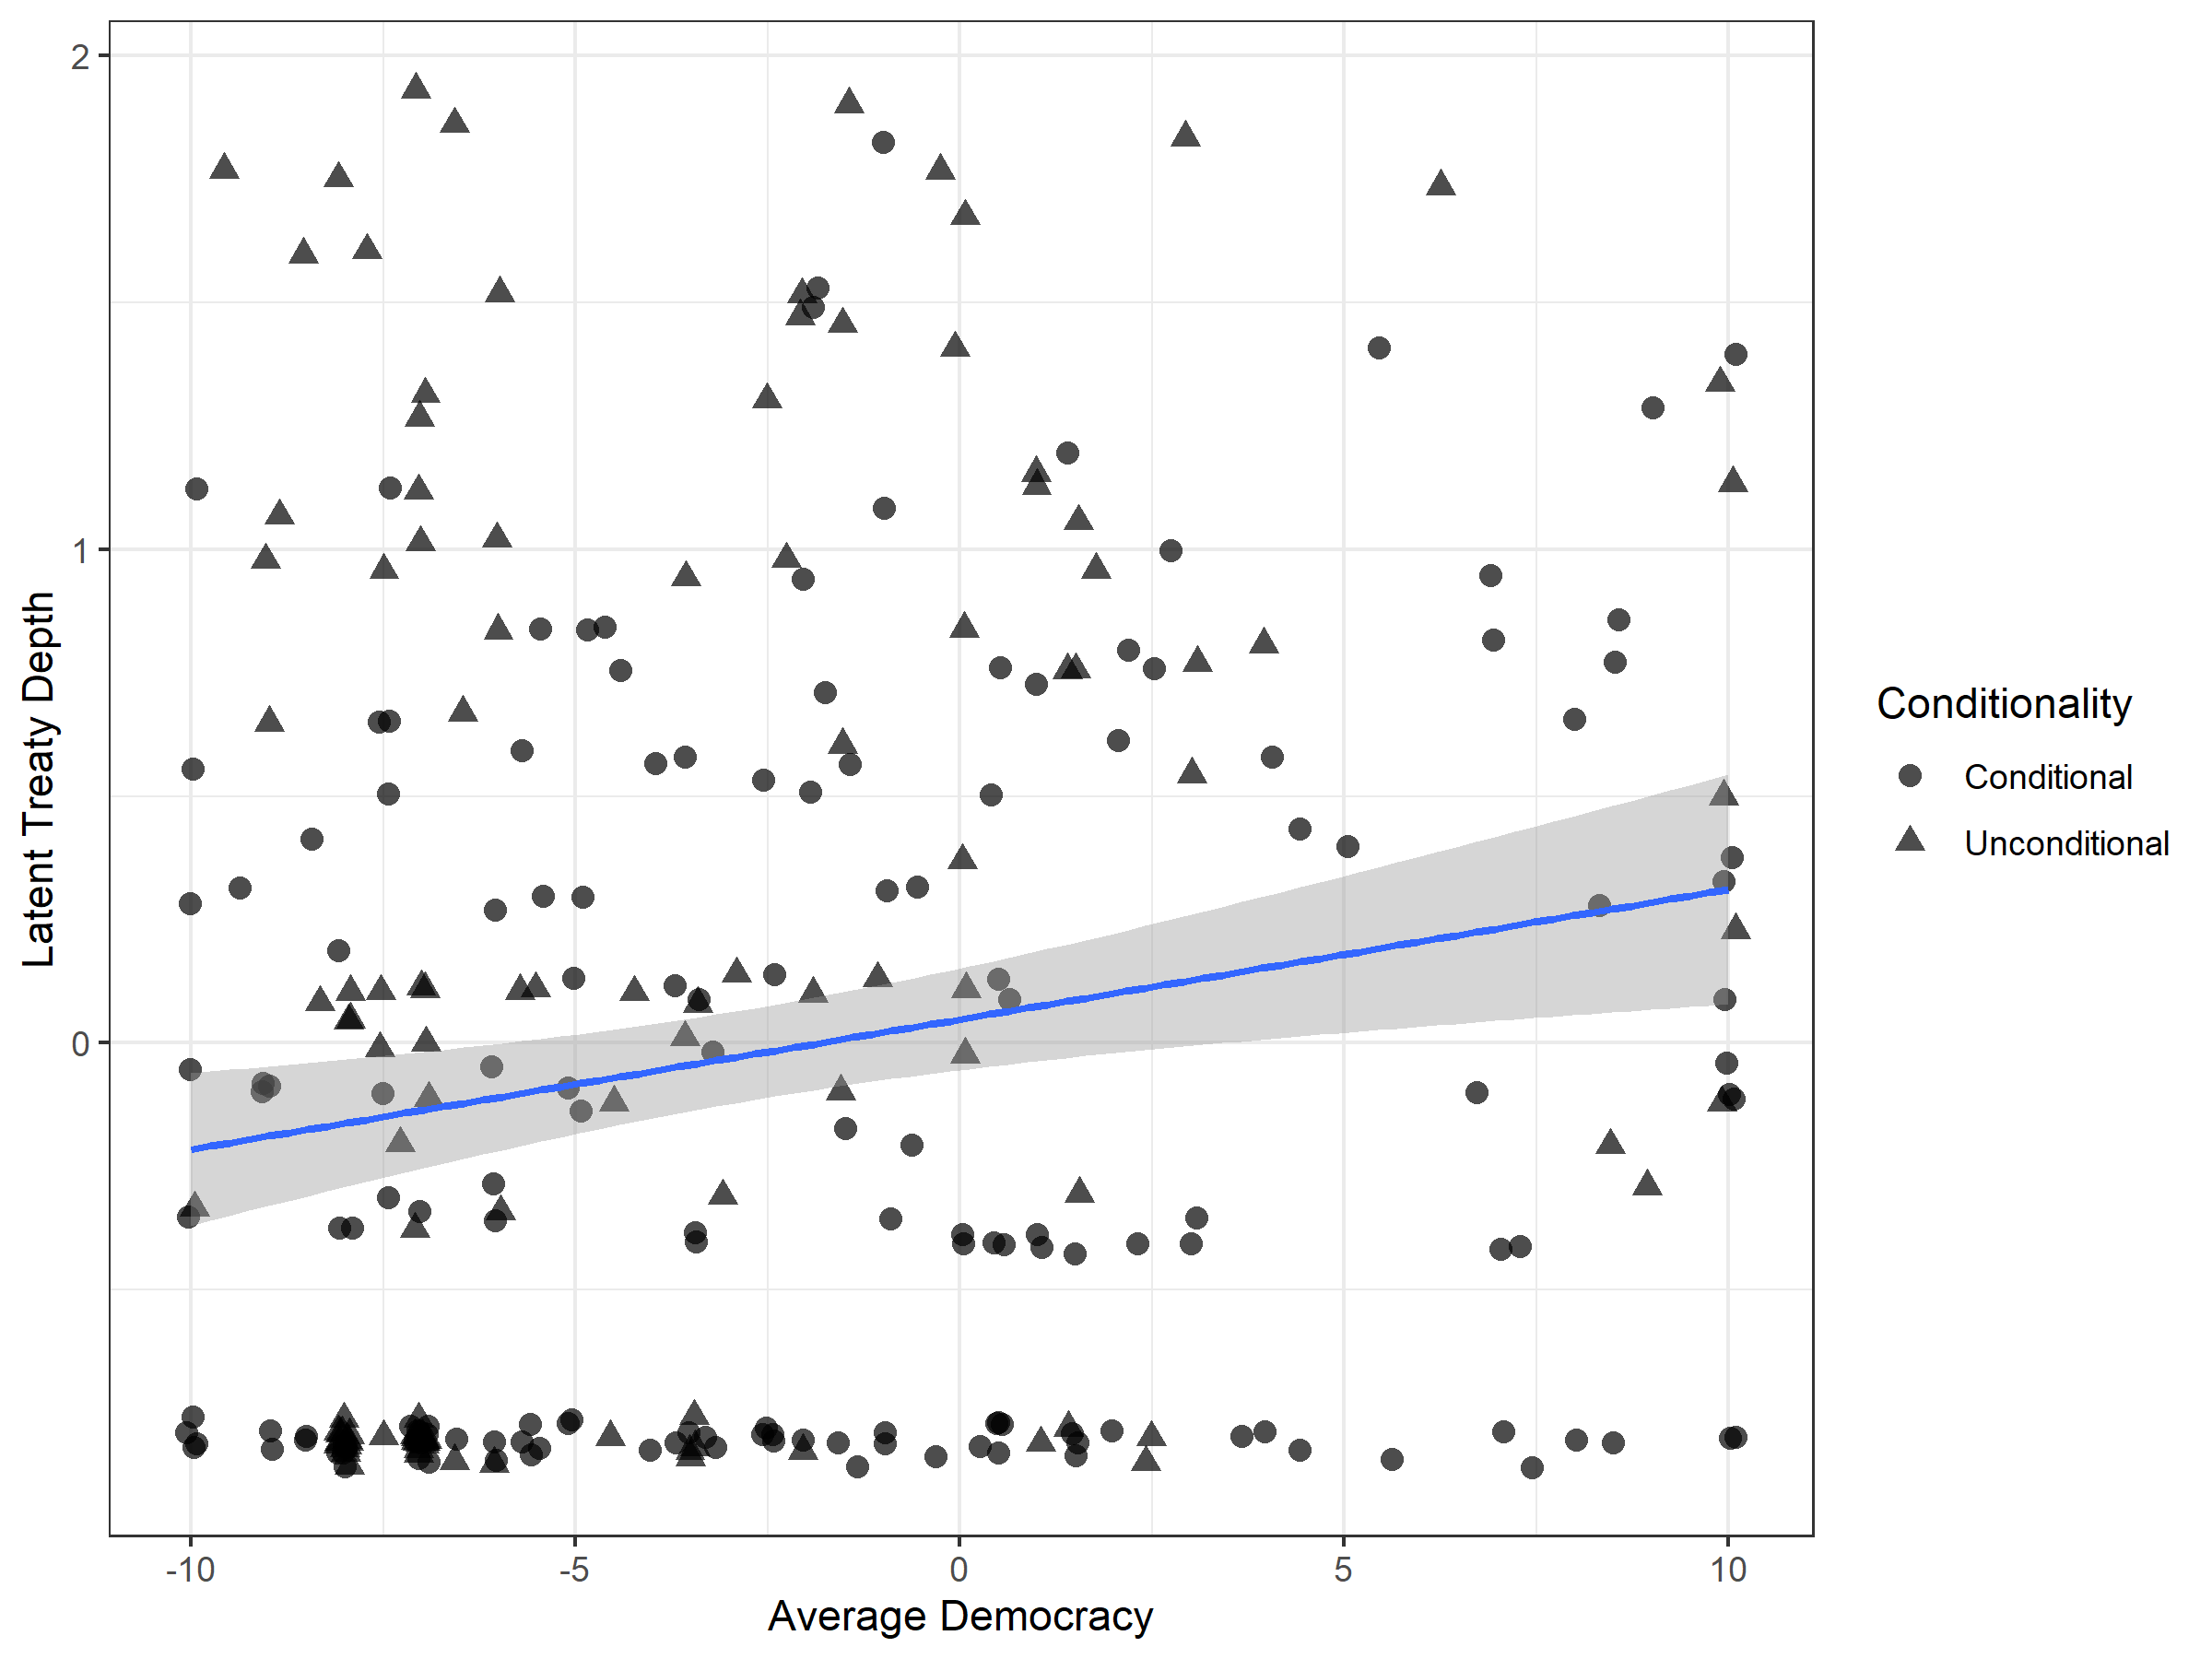
\includegraphics[width=0.68\textwidth]{../figures/democ-combo.png}
\caption{Average of the most capable alliance member's Polity score when the alliance formed in four groups of alliance from 1816 to 2007. Divisions between alliances based on unconditional military support and treaty depth. Darker quadrants mark a higher average democracy score for that group of alliances, and the text in each box gives the precise value.}
\label{fig:democ-combo}
\end{figure}


These descriptive results do not adjust for potential confounding factors, however.
Therefore, I describe results from statistical models of depth and unconditional military support, starting with separate models. 
\autoref{tab:separate-models} shows results from a beta model of treaty depth and a binomial model of unconditional military support with a probit link function. 
The results are partially consistent with the hypotheses.
First, I find a positive association between the democracy of the most capable alliance member and treaty depth. 
For unconditional military support, the parameter estimate is negative, but the 95\% confidence interval for alliance leader democracy includes zero and positive values. 


\begin{table}[!htbp] \centering 
  \caption{Independent Models of Alliance Treaty Depth and Unconditional Military Support in ATOP Offensive and Defensive Alliances from 1816 to 2007.} 
  \label{tab:separate-models} 
\begin{tabular}{@{\extracolsep{5pt}}lcc} 
\\[-1.8ex]\hline 
\hline \\[-1.8ex] 
 & \multicolumn{2}{c}{\textit{Dependent variable:}} \\ 
\cline{2-3} 
\\[-1.8ex] & Latent Depth (rescaled) & Unconditional Military Support \\ 
\\[-1.8ex] & \textit{beta} & \textit{probit} \\ 
\\[-1.8ex] & (1) & (2)\\ 
\hline \\[-1.8ex] 
  Alliance Leader Polity & 0.023$^{}$ & $-$0.018 \\ 
  & (0.002, 0.043) & ($-$0.047, 0.011) \\ 
  Foreign Policy Concessions & $-$0.057 & 0.021 \\ 
  & ($-$0.209, 0.096) & ($-$0.197, 0.239) \\ 
  Number of Members & 0.016 & $-$0.030 \\ 
  & ($-$0.011, 0.043) & ($-$0.077, 0.018) \\ 
  Wartime Alliance & $-$0.309$^{}$ & $-$0.954$^{}$ \\ 
  & ($-$0.658, 0.040) & ($-$1.570, $-$0.338) \\ 
  Asymmetric Obligations & 0.189 & 0.035 \\ 
  & ($-$0.155, 0.532) & ($-$0.467, 0.537) \\ 
  Asymmetric Capability & 0.347 & 0.651 \\ 
  & ($-$0.120, 0.814) & ($-$0.218, 1.520) \\ 
  Non-Major Only & 0.275 & 1.146$^{}$ \\ 
  & ($-$0.228, 0.779) & (0.266, 2.027) \\ 
  Average Threat & 1.248$^{}$ & 1.630$^{}$ \\ 
  & (0.376, 2.120) & (0.295, 2.965) \\ 
  Foreign Policy Disagreement & 0.197 & 0.394 \\ 
  & ($-$0.258, 0.653) & ($-$0.306, 1.094) \\ 
  Start Year & 0.004$^{}$ & 0.015$^{}$ \\ 
  & (0.0004, 0.007) & (0.010, 0.021) \\ 
  Constant & $-$8.929$^{}$ & $-$31.655$^{}$ \\ 
  & ($-$15.679, $-$2.179) & ($-$43.220, $-$20.091) \\ 
 \hline \\[-1.8ex] 
Observations & 277 & 277 \\ 
Log Likelihood & 54.349 & $-$132.467 \\ 
\hline 
\hline \\[-1.8ex] 
\textit{Note:}  & \multicolumn{2}{r}{95\% Confidence Intervals in Parentheses.} \\ 
\end{tabular} 
\end{table} 


I use the coefficient estimates in \autoref{tab:separate-models} to assess the substantive impact of alliance leader democracy in \autoref{fig:results-democ-max}.
This figure plots the predicted value of both outcomes based on the alliance leader's Polity score. 
The left-hand plot of \autoref{fig:results-democ-max} shows the association between the democracy of the most capable alliance member and the predicted probability of unconditional military support. 
This relationship is weaker than expected.  
These results diverge from previous findings that democratic alliance membership leads to limited obligations \citep{Mattes2012, Chibaetal2015}, perhaps due to a different sample of alliances, different model specifications, and my emphasis on the alliance leader. 


\begin{figure}[hbtp]
\centering
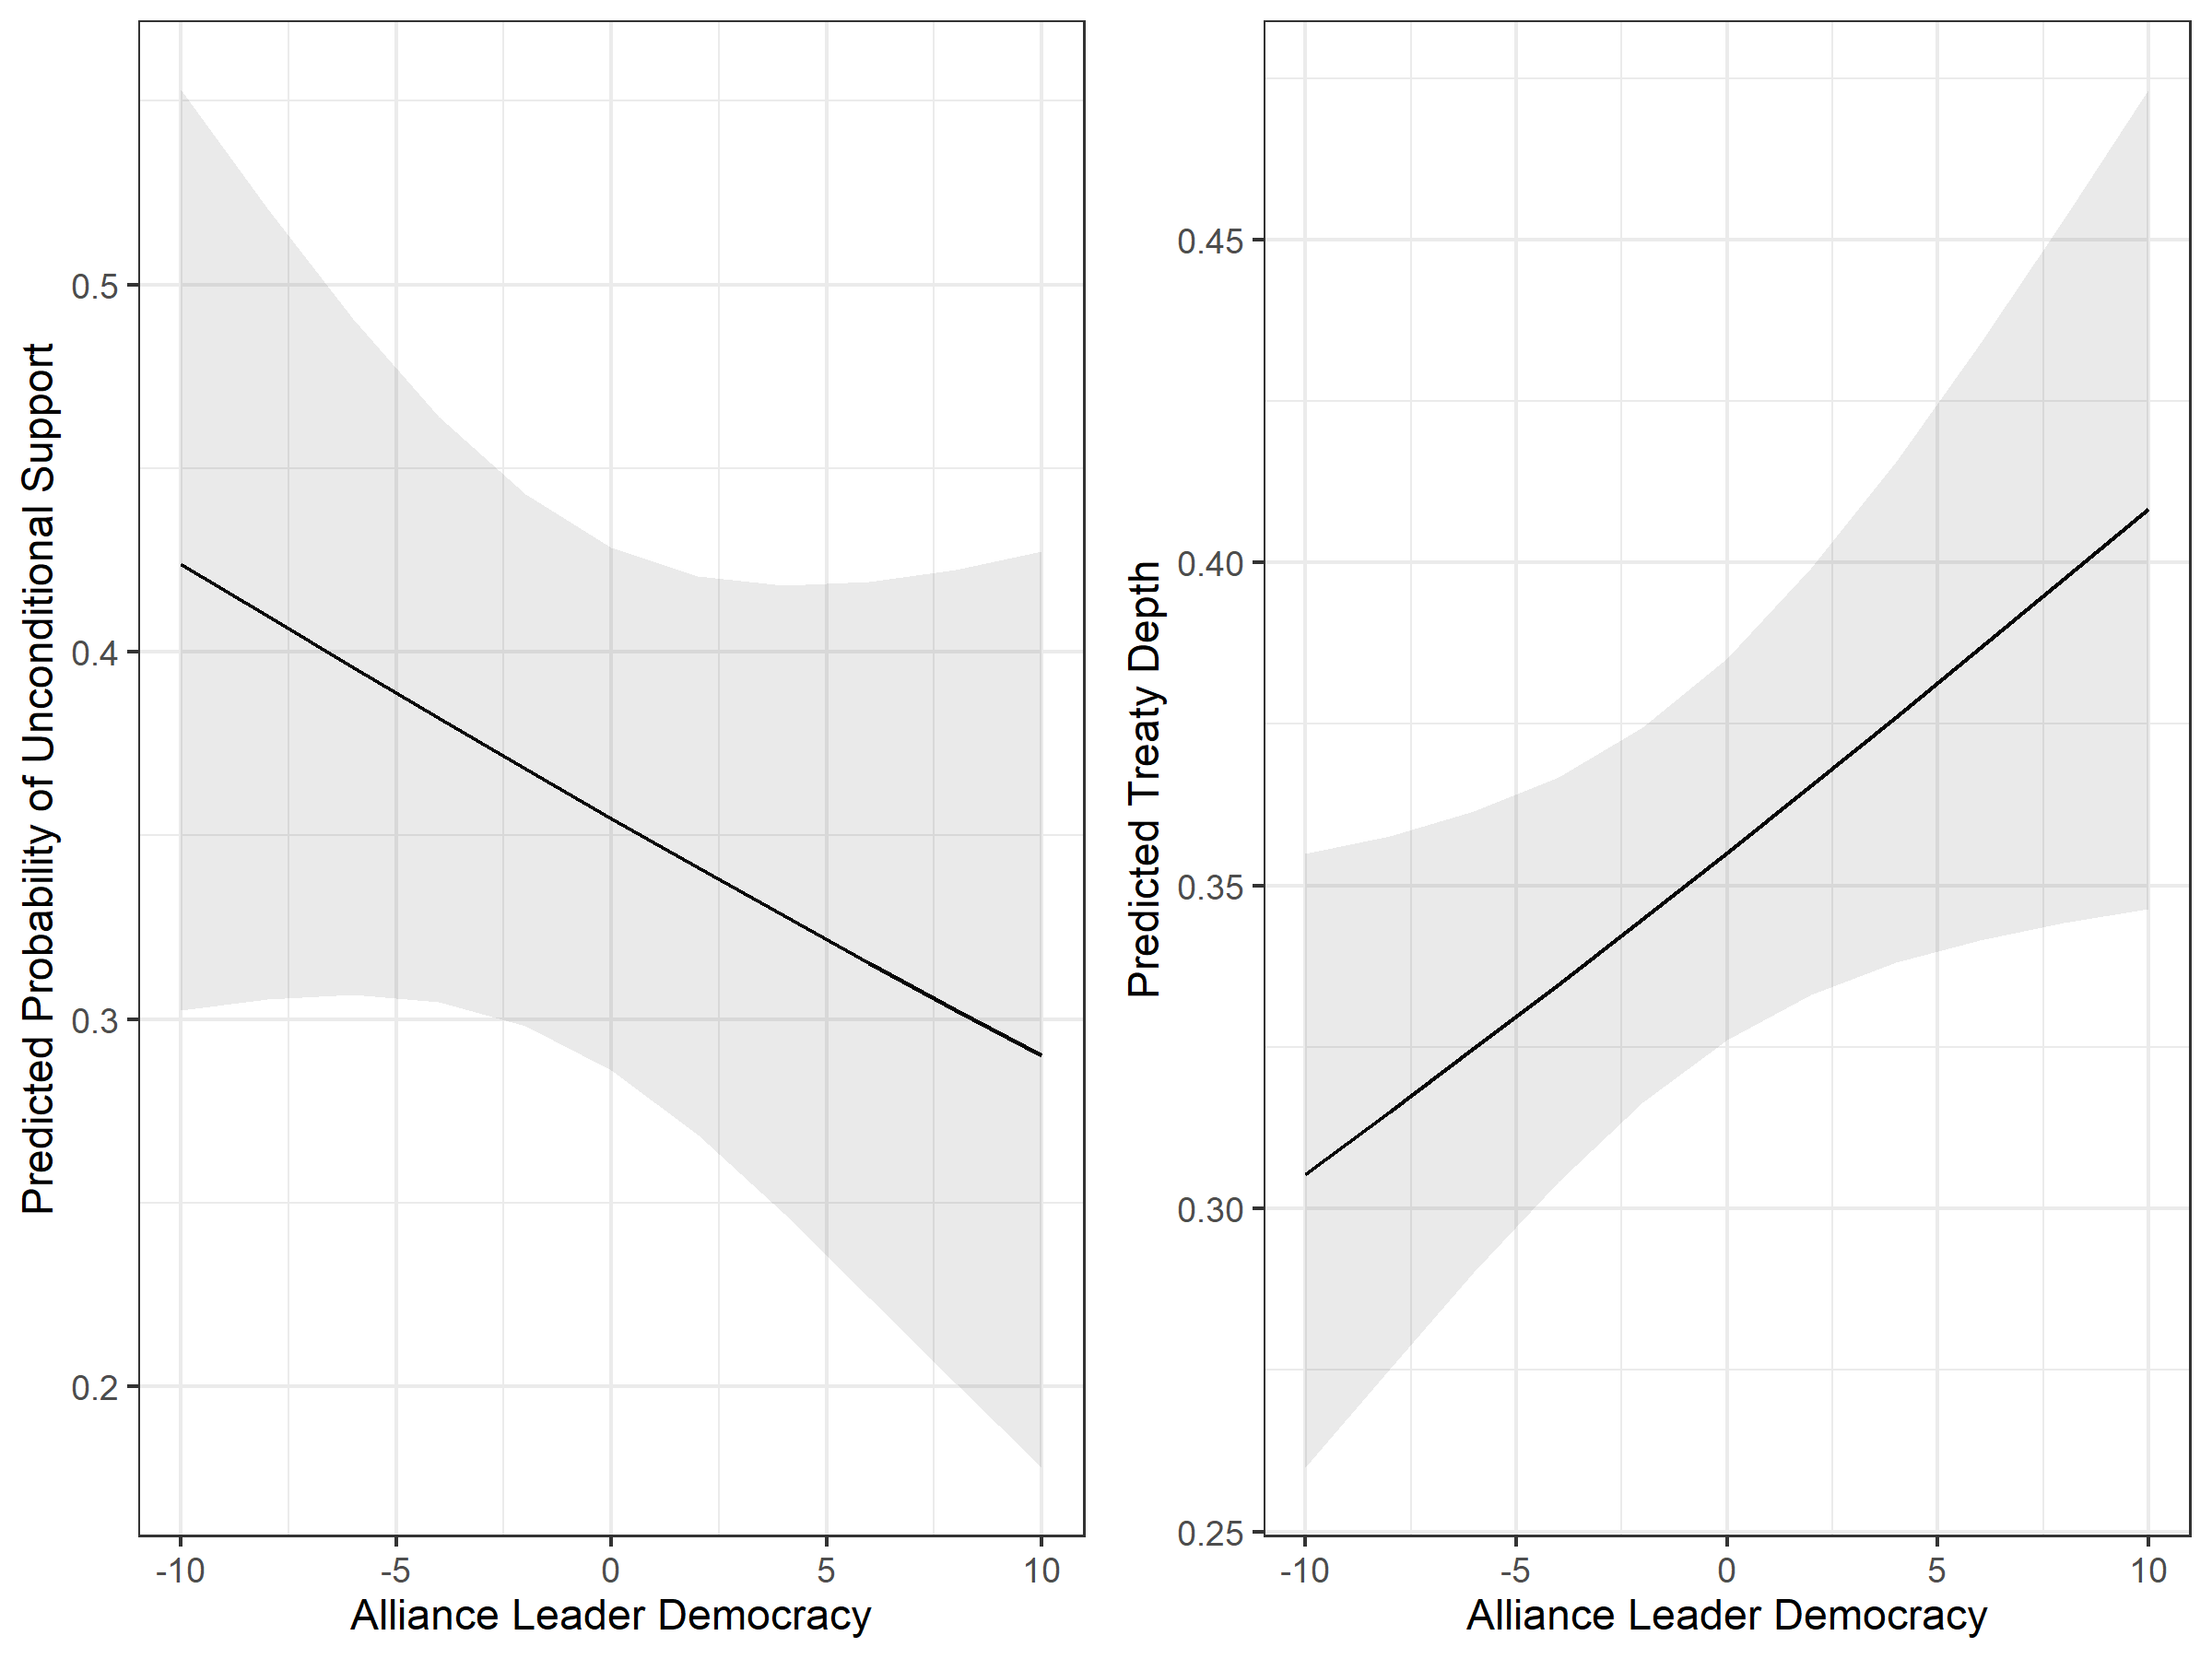
\includegraphics[width=0.95\textwidth]{../figures/results-democ-max.png}
\caption{Predicted probability of unconditional military support and predicted treaty depth across the range of alliance leader Polity scores. The line marks predicted values, and the shaded areas encapsulate the standard errors. Predictions based on coefficient estimates from probit and beta regression models, holding all other variables at their mode or median.}
\label{fig:results-democ-max}
\end{figure}


The right-hand plot in \autoref{fig:results-democ-max} shows a positive relationship between alliance leader democracy and treaty depth.
Alliances with a democratic leader have greater treaty depth, all else equal. 
In expectation, the predicted value of rescaled treaty depth in an alliance with a fully democratic leader is roughly .1 greater than an alliance with a fully autocratic leader. 
As rescaled depth ranges between 0 and 1, this is a substantively large relationship that matches the treaty depth hypothesis.


Although the results from separate models are informative, they do not account for correlations in the error terms of the depth and unconditional support models, which could affect inferences. 
I now report the results of a bivariate model of depth and unconditional military support in \autoref{tab:gjrm-res}. 
This table contains results from both equations of the GJRM.\footnote{I mark smoothed terms with the letter s.}
As in \autoref{tab:separate-models}, I find a positive relationship between the democracy of the leading alliance member and treaty depth, but a weak negative relationship between democratic influence and treaty depth.  
The control variables in this model are also interesting and somewhat different from the univariate models.  
Asymmetric capability and the number of alliance members both increase depth. 
Asymmetric capability in an alliance and symmetric alliances between non-major powers are more likely to include unconditional military support than symmetric major power alliances. 
I also find that alliances with more members and wartime treaties have a lower probability of unconditional military support. 
Last, threat and the year of alliance formation increase unconditional military support and treaty depth. 


\begin{table}[ht]
\centering
\begin{tabular}{lrrrr}
  & \multicolumn{2}{c}{Uncond. Mil. Support} & \multicolumn{2}{c}{Latent Depth}\\ \hline
  & Estimate & Std. Error & Estimate & Std. Error \\ 
  \hline
  Alliance Leader Polity & -0.0173979 & 0.0158094 & 0.0262429 & 0.0097732 \\ 
  Economic Issue Linkage & 0.2232389 & 0.2006227 & -0.0060972 & 0.1458203 \\ 
  FP Concessions & -0.1468542 & 0.1214414 & -0.0339923 & 0.0845875 \\ 
  Number of Members & -0.0994788 & 0.0264666 & 0.0179032 & 0.0129499 \\ 
  Wartime Alliances & -0.6274650 & 0.3157751 & -0.0744869 & 0.1787959 \\ 
  Asymmetric Obligations & -0.0181268 & 0.2622665 & 0.1686232 & 0.1632100 \\ 
  Asymmetric Capability & 0.9586816 & 0.3864164 & 0.3436770 & 0.2192153 \\ 
  Non-Major Only & 1.7040882 & 0.3975041 & 0.0828621 & 0.2310327 \\ 
  FP Disagreement & 0.1253382 & 0.3352438 & 0.3284441 & 0.2204690 \\ 
  s(Mean Threat) & 7.3253441 & 43.4564525 & 1.0000004 & 16.8780421 \\ 
  s(Start Year) & 4.7057429 & 49.8605879 & 3.3275472 & 39.7155651 \\
  (Intercept) & -1.0980618 & 0.4635789 & -1.0810691 & 0.2485382 \\  
   \hline
\end{tabular}
\caption{Results from joint generalized regression model of treaty depth and unconditional military support. 
              Sample is offensive and defensive alliances from 1816 to 2007.
                     All smoothed terms report the effective degrees of freedom and the chi-squared term. 
                     The unconditional military support model is a binomial GLM with a probit link function. 
                     The treaty depth model is a beta regression. 
                     I model the error correlation between the two processes with a T copula.} 
\label{tab:gjrm-res}
\end{table} 


Univariate and bivariate models generate similar inferences about democractic alliance leadership and treaty design.
The Polity score of the most capable alliance member is positively correlated with treaty depth, but has at most a slight negative association with unconditional military support.
Inferences about the control variables vary somewhat across the two models, however, which suggests that accounting for correlated errors is worthwhile.   



\subsection{Elections, Political Competition and Executive Constraints} 


Having analyzed aggregate democracy scores, I now distinguish between the three components of the Polity index. 
The key independent variables in this model are binary indicators of competitive elections, open political competition, and executive constraint through parity or subordination to other actors. 
All three factors could expose leaders to scrutiny of their foreign policy decisions and audience costs. 
I use a bivariate GJRM to estimate these effects.\footnote{A T copula has the best model fit and AIC.} 


\begin{table}[ht]
\centering
\begin{tabular}{lrrrr}
 & \multicolumn{2}{c}{Uncond. Mil. Support} & \multicolumn{2}{c}{Latent Depth}\\ \hline
   & Estimate & Std. Error & Estimate & Std. Error \\ 
  \hline 
  Competitive Elections & -1.3862036 & 0.5969913 & 1.0334447 & 0.3441959 \\ 
  Political Competition & 0.1267747 & 0.4456283 & -0.3968825 & 0.2894709 \\ 
  Executive Constraints & 0.7810824 & 0.2758115 & -0.3806161 & 0.2006471 \\ 
  Economic Issue Linkage & 0.0786646 & 0.1830420 & 0.1099506 & 0.1466334 \\ 
  FP Concessions & -0.1284395 & 0.1256934 & -0.1052689 & 0.0817796 \\ 
  Number of Members & -0.1004983 & 0.0271633 & 0.0268154 & 0.0139085 \\ 
  Wartime Alliances & -0.7495699 & 0.2448796 & 0.0599420 & 0.1700357 \\ 
  Asymmetric Obligations & -0.0230173 & 0.2251492 & 0.1766837 & 0.1620580 \\ 
  Asymmetric Capability & 1.0281801 & 0.5255088 & 0.4985258 & 0.2426731 \\ 
  Non-Major Only & 1.6291469 & 0.5180102 & 0.1175974 & 0.2551236 \\ 
  FP Disagreement & 0.1726706 & 0.2975962 & 0.3405041 & 0.2124881 \\ 
  s(Mean Threat) & 7.5870610 & 44.8092434 & 1.0000005 & 25.8169433 \\ 
  s(Start Year) & 5.9742148 & 50.0279652 & 8.3362695 & 57.7689902 \\ 
  (Intercept) & -0.8925660 & 0.6081549 & -1.3310577 & 0.2833844 \\
   \hline
\end{tabular}
\caption{Results from joint generalized regression model of treaty depth and unconditional military support as a function of competitive elections, political competition and executive constraints in the most capable alliance member.
              Sample is offensive and defensive alliances from 1816 to 2007.  
                     All smoothed terms report the effective degrees of freedom and the chi-squared term. 
                     The unconditional military support model is a binomial GLM with a probit link function. 
                     The treaty depth model is a beta regression. 
                     I model the error correlation between the two processes with a T copula.} 
\label{tab:gjrm-res-split}
\end{table}


The three components of democracy have different consequences for alliance treaty design.
First, elections decrease the probability of unconditional military support and increase treaty depth.
This matches the argument--- if leaders can be removed from office by competitive elections, they prefer treaty depth to unconditional military support because depth is less salient for voters. 
Second, the political competition coefficient for treaty depth is negative, albeit with substantial uncertainty. 
This implies that scrutiny of the executive from open political competition may restrain deep alliance commitments, but the effect is unclear. 
Political competition has no clear association with the probability of unconditional military support. 


Last, executive constraints has the opposite effect of electoral competition on both credibility sources, which is interesting and unexpected, so I offer brief ex post explanations.
First, I find that executive constraints reduce treaty depth.  
Constraints might reduce treaty depth by exposing the executive to scrutiny from other political elites who have ample foreign policy information and want to avoid foreign entanglements.  
Second, domestic institutions with executive parity or subordination increase the probability of unconditional military support.  
One explanation for the positive relationship between constraints and unconditional support is that democratic leaders attempt to commit successors with different foreign policy preferences to the alliance \cite{Mattes2012a}. 
Leadership turnover in democracies threatens international cooperation, because new leaders may have different supporters and preferences \citep{Lobell2004, Narizny2007, Leedsetal2009}. 
By making an unconditional promise of military support, leaders force successor governments to pay higher audience costs to break the alliance. 


Taken together, the results from dividing democratic institutions may explain the aggregate democracy findings. 
The large effect of competitive elections drives the overall positive association between democracy and treaty depth, as it overwhelms the slight negative effect of executive constraints. 
Competitive elections and executive constraints have offsetting effects on the probability of unconditional military support. 
Therefore, I find a weak association between the democracy of the alliance leader and the probability of unconditional military support. 
Keeping these patterns in mind, I now examine the North Atlantic Treaty Organization (NATO) to illustrate the theoretical process. 


\subsection{NATO Treaty Design}


I use NATO to show the theoretical mechanisms for two reasons. 
First, the process behind NATO applies to multiple alliances, as other US alliance treaties have similar designs. 
Second, NATO is the most important alliance in international politics, as it has played a crucial role in the structure of international relations since 1949. 
Because NATO is an exceptionally durable and consequential alliance, understanding how the treaty formed is worthwhile. 


After World War II, the United States sought a way to protect Europe from the USSR. 
Despite acute security concerns, fear of entrapment in unwanted conflicts led the United States to place limits on military support. 
As \citet{Poast2019a} details, NATO members disagreed over how to define the North Atlantic area, especially with reference to France's Algerian colony and Italy, as the North Atlantic area was a key condition on military support. 
Furthermore, active military support from NATO members depends on domestic political processes.\footnote{\citet{Benson2012} calls this commitment a ``probablistic'' obligation.} 
Isolationists in the US Senate feared that an alliance would force America to intervene automatically if partners were attacked, bypassing the power of Congress to declare war and engaging the US in unwanted conflicts \citep[pg. 280-1]{Acheson1969}.
Therefore, Article V of the NATO treaty states that if one member is attacked the others ``will assist the Party or Parties so attacked by taking forthwith, individually and in concert with the other Parties, \emph{such action as it deems necessary} (emphasis mine).'' 
Military support was and is not guaranteed by Article V. 
Secretary of State Dean Acheson stated as much in a March 1949 press release defending NATO to the US public, where he said that Article V ``does not mean that the United States would automatically be at war if one of the nations covered by the Pact is subject to armed attack'' \citep{Acheson1949}.
This claim and the emphases of the press release shows that promises of military support were salient to the US public and that entrapment concerns of US leaders led to limited promises of military support. 


Military support from Article V did not assuage European fears that if the Soviets invaded, the United States would not fight. 
To increase the credibility of NATO, the United States took other measures.  
A 1951 presentation by Dean Acheson to Dwight Eisenhower argued that European allies ``fear the inconstancy of United States purpose in Europe. ... These European fears and apprehensions can only be overcome if we move forward with determination and if we make the necessary full and active contribution in terms of both military forces and economic aid'' \citep[pg. 3]{Acheson1951}. 
To start, the US supported the Atlantic Council, an international organization and the main source of depth in the NATO treaty. 
The United States used the Atlantic Council to coordinate collective defense and increase the perceived reliability of the alliance. 
By investing in the Atlantic Council and related joint military planning, the US addressed European fears of abandonment. 
For example, US officials thought that the British Foreign Minister viewed US provision of a supreme commander in Europe as ``a stimulus to European action'' in NATO \citep{Acheson1950}. 


Many Senators also opposed military aid to Europe \citep[pg 285]{Acheson1969}, which constrained further treaty depth. 
Thus, legislative constraints on the executive branch reduced the formal depth of NATO relative to what many ambassadors preferred \citep[pg 277]{Acheson1969}, which matches the statistical inference about executive constraints and treaty depth.  
Bilateral agreements on troop deployments thus became another instrument of reassurance. 
In 1950 the Germans formally requested clarification on whether an attack on US forces in Germany would be treated as an armed attack on the United States- and US policymakers said that it would \citep[pg. 395]{Acheson1969}.  
These bilateral arrangements and basing rights are not covered in the NATO treaty, but they added substantial depth.\footnote{This reveals a potential limitation of the statistical models.}  


% Sum up 
In NATO, fear of entrapment led the United States to offer conditional military support, but did not inhibit deep military cooperation, which helped reassure European allies. 
Limits on the promises of military support were a salient part of public discussions in the NATO treaty, while the Atlantic Council had a smaller role in public discourse. 
The Atlantic Council and associated bureaucratic machinery are the formal core of substantial defense cooperation. 
NATO negotiations show how a democratic alliance leader used treaty depth to reassure their allies, rather than unconditional military support. 
In the next section, I summarize some implications of the results and offer concluding thoughts. 



\section{Discussion and Conclusion} 


% main evidence for an indirect effect
In summary, the findings from the statistical models generate mixed evidence for the hypotheses, and the NATO illustration suggests that the theoretical mechanisms are plausible. 
I find consistent evidence that democracies design deep alliances, and that this relationship may be driven by electoral politics.  
Because democratic leaders are concerned with audience costs and foreign entanglement from treaty depth has little electoral salience, democracies often use depth to increase the credibility of their alliances.
There is inconsistent support for the claim that allied democracy decreases the probability of unconditional military support, however, because competitive elections and executive constraints have contradictory effects. 
Elections encourage conditional obligations to address audience cost concerns, but executive constraints may encourage attempts to lock successors into the alliance with unconditional support.
Inasmuch electoral politics are a key source of audience costs, the results are largely consistent with my claim that states form deep alliances to increase the credibility of their alliance commitments while managing entrapment risk and audience costs.


% limitations
My argument and evidence has two limitations.
First, I only examine variation in formal treaty design. 
This omits treaty implementation, which can diverge from the formal commitment.   
Formal treaty depth often reflects practical depth, but it may miss some differences between alliances. 
Changes in realized alliance depth are a useful subject for future inquiry, but will require extensive data collection.
Second, I examine 280 alliances, which is a small sample. 
Inferences from small samples can be more sensitive to model and data changes, which could explain why my inferences differ from previous studies. 
For example, I use a more recent version of the ATOP data than \citet{Chibaetal2015}, which could explain our divergent findings about democracy and conditionality in alliances with active military support. 


Despite its limitations, this paper has three main implications for scholarship. 
First, treaty depth shapes alliance politics. 
Alliance members can use treaty depth to avoid trading credibility for entrapment risk, albeit at the cost of greater foreign entanglement. 
When depth substitutes for unconditional military support, alliances with conditional obligations may lose little credibility.  


Second, democracies do not make limited alliance commitments. 
A fully limited alliance has conditional obligations and no depth.
Even if democracies impose conditions on military support, deep alliances add substantial foreign entanglement, so many democratic alliances are not completely limited.  
Third, some of the lessons from this work add to the extensive literature on the design on international institutions \citep{DownesRocke1995, MartinSimmons1998, Koremenosetal2001, Thompson2010}.
In the same way that democracies use depth to support allies while managing electoral politics, democracies may undertake deep international commitments in ways that limit public scrutiny. 


The findings raise at least two questions for future research.  
For one, they speak to debates about whether democracies make more credible commitments. 
The net effect of democracy on alliance credibility includes conditions on military support, treaty depth, and the direct effect of institutions and domestic politics. 
These three mechanisms may have competing or conditional effects, which could explain mixed findings about the credibility of democratic commitments \citep{Schultz1999, Leeds1999, Thyne2012, DownesSechser2012, PotterBaum2014}.
Treaty design also reinforces strategic selection problems in testing audience costs \citep{Schultz2001}. 
Future research should combine the components of democracy and democratic alliances to asses the net effect of democracy on credible commitment in international relations. 


Scholars should also consider how alliance treaty design varies across different types of autocracies. 
As I noted in the argument, some autocratic states have high audience costs for backing down in military interventions. 
Differences in the salience of audience costs, which actors impose audience costs on leaders and what information those actors have about foreign policy \citep{Weeks2008} may help explain alliance treaty design.
For example, personalist leaders with few public or elite constraints on their foreign policy may design alliances with depth and unconditional military support. 


In conclusion, states use deep alliances to reassure their partners while limiting entrapment risk and exposure to audience costs. 
By shaping leaders' foreign policy audiences and audience cost concerns, domestic political institutions influence how states build credibility into alliance treaties.
Due to high audience costs and limited public scrutiny of foreign entanglements, democracies use treaty depth to increase the credibility of their alliances. 



 
\bibliography{../../../MasterBibliography} 





\end{document}
